\documentclass[11pt]{article}
\usepackage{amsmath,amsfonts,amssymb}
\usepackage{hyperref}
\hypersetup{
	colorlinks=true,
	linkcolor=blue,
	urlcolor=cyan
	}
\usepackage[margin=1in]{geometry}
\usepackage{graphicx}

\setlength{\parindent}{0pc}
\setlength{\parskip}{10pt}

\newcommand{\solution}[1]{{\color{blue} \textit{Solution} : #1}}
%%%%%%%%%%%%%%%%%% TO REMOVE SOLUTION %%%%%%%%%%%%%%%%%%
% \renewcommand{\solution}[1]{}


\title{STAT 165/265 HW 3}
% \date{Jan 31, 2024}

\begin{document}

\maketitle

\hfill \textbf{Submit to Gradescope by Tuesday, February 11 at 11:59pm}
\section*{Deliberate Practice: Zeroth and First Order Forecasting}

\emph{Expected completion time: 60 minutes} \\
\emph{Graded on completion \& using the correct relative error formula}

For each of the following time series, estimate the value of the next few points without looking things up, then look at your answers and report your relative errors. Try to be accurate, even if you don't use a zeroth/first order forecast for each question. Just write down your answer and relative error for each question (no need to show work). When you have answered all the questions, write 1-2 paragraphs summarizing which strategies worked well and which strategies worked poorly.

\begin{enumerate}
	\item United States energy usage
	
	\begin{itemize}
          \item Find the graph by going to \href{https://www.eia.gov/electricity/gridmonitor/expanded-view/electric_overview/US48/US48/ElectricityOverview-2/edit}{this link}. In ``Chart options'' and ``Date Range Type'' select ``Custom'', in ``Date Range'' enter ``01/01/2025 - 01/21/2025'', and switch the time zone to Pacific.
          \item Predict what the energy usage was on 01/26/2025 at 4pm Pacific time.
          \item After you've made your prediction, extend the date range to find the true answer.
	\end{itemize}
	
	\item Number of full-time Facebook/Meta employees until 2016
	
	\begin{center}	
		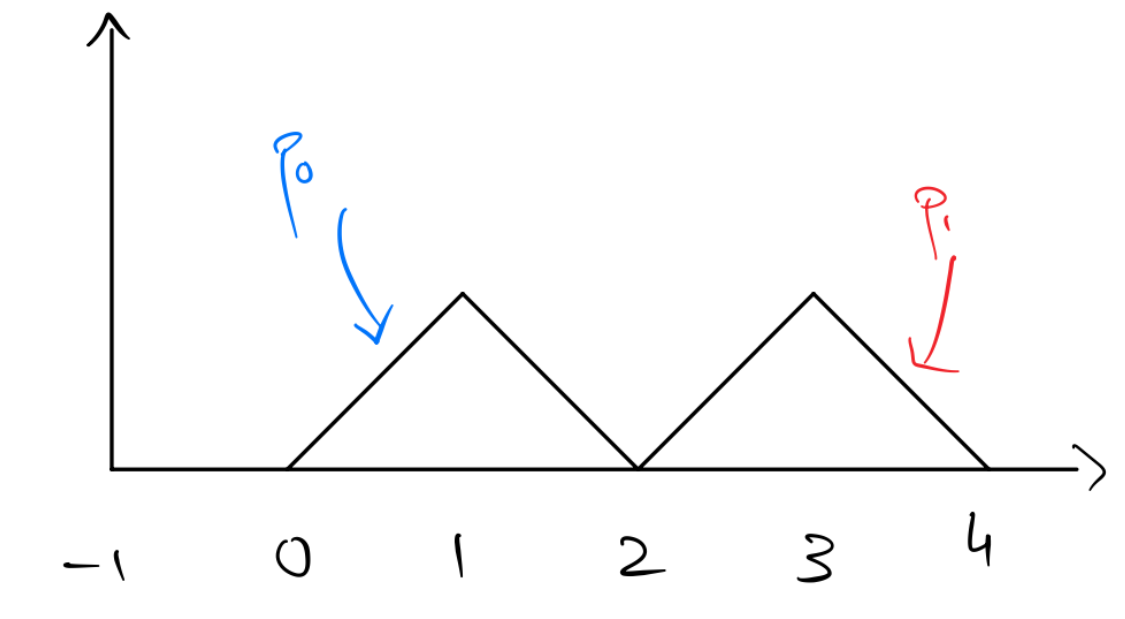
\includegraphics[width = 375px]{2.png}
	\end{center}

	\begin{itemize}
		\item Predict the number of full-time employees in 2018 and 2020.
            \item After you've made your prediction, check your answers at \href{https://www.globaldata.com/data-insights/technology--media-and-telecom/metas-employee-headcount/}{this link}. Report your relative error for each of the years requested.
	\end{itemize}
	
	\item Total adult correctional population until 2010

	\begin{center}	
		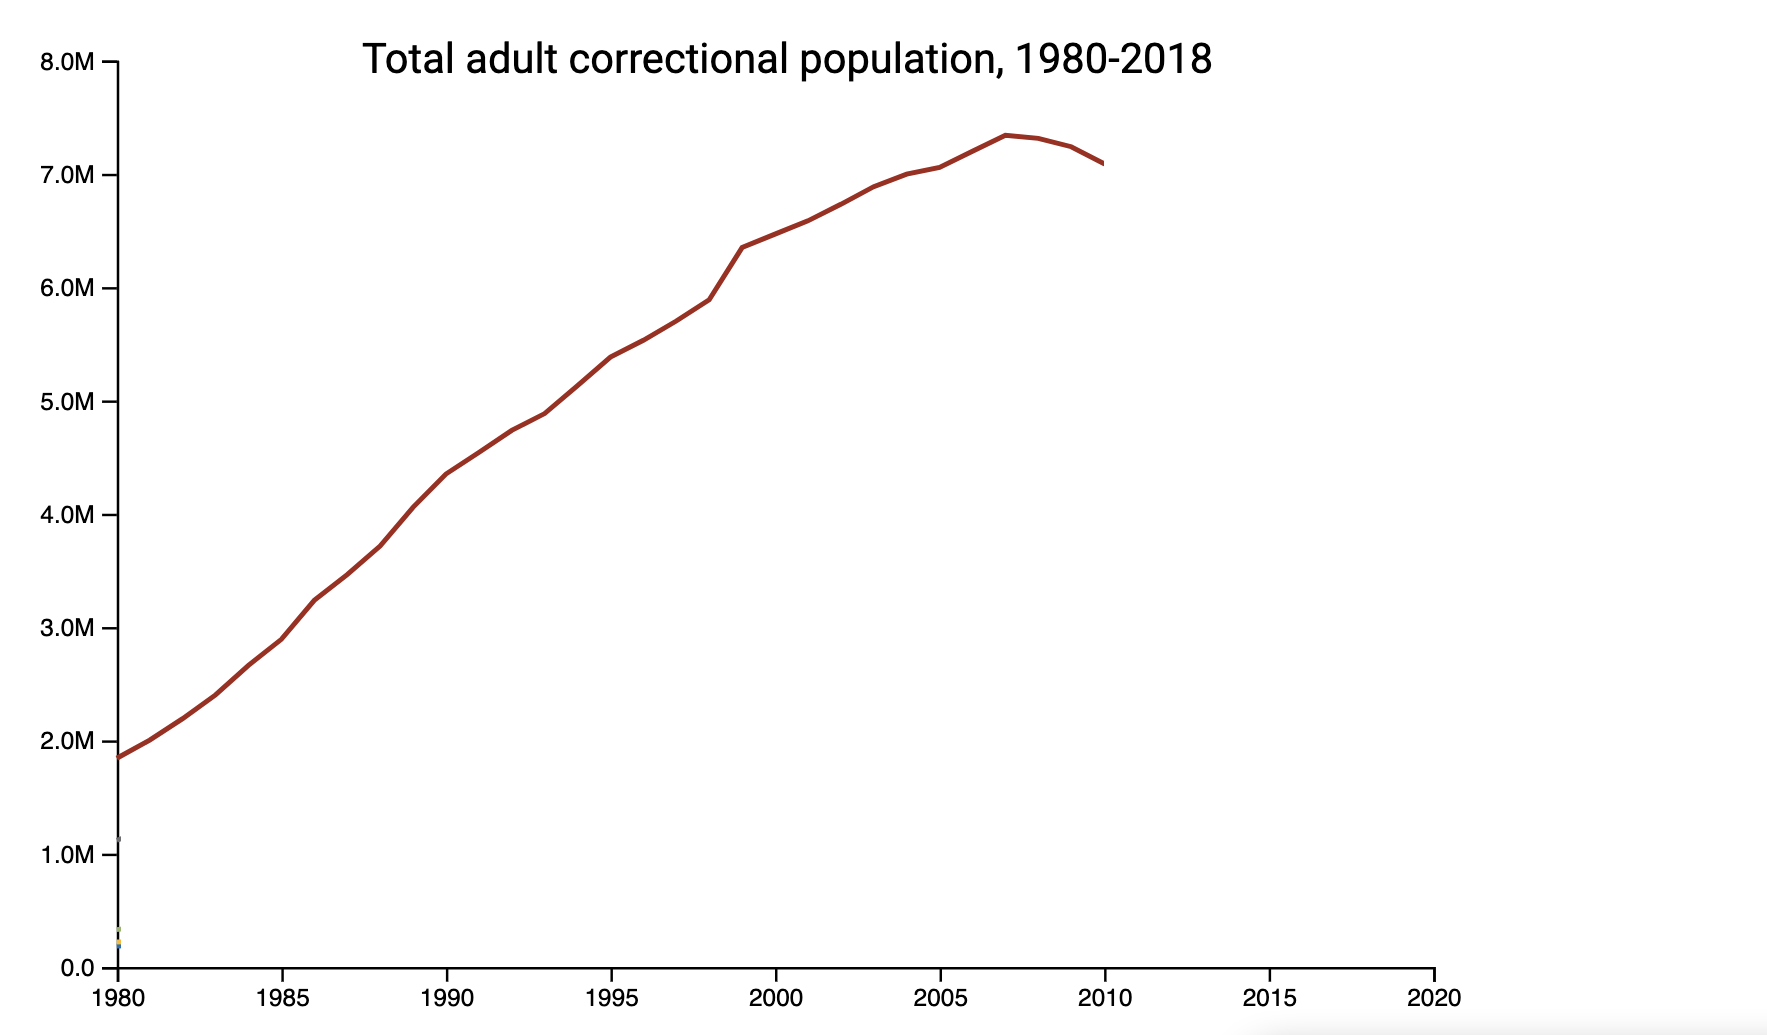
\includegraphics[width = 375px]{3.png}
	\end{center}


	\begin{itemize}
		\item Predict the adult correctional population in 2014 and 2018.
            \item After you've made your prediction, check your answers at \href{https://bjs.ojp.gov/data/key-statistics#total-correction-population}{this link}. Report your relative error for each of the years requested.
	\end{itemize}
	
	\item World GDP until 1950
	\begin{itemize}
		\item Find the graph by going to \href{https://ourworldindata.org/grapher/world-gdp-over-the-last-two-millennia?time=1..1950}{this link}.
		\item Predict World GDP in 1960, 1970, and 1990.
            \item After you've made your predictions, move the slider at the bottom to reveal the correct answers. Report your relative error for each of the years requested.
	\end{itemize}
	
	\item TSA passenger throughput

	\begin{center}	
		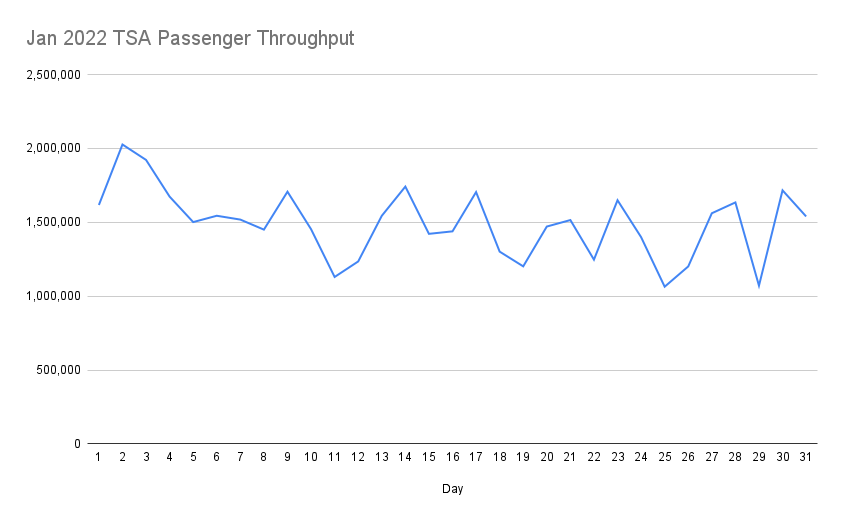
\includegraphics[width = 375px]{tsa_checkpoint2.png}
	\end{center}

	\begin{itemize}
		\item This graph shows TSA checkpoint throughput for January 2022.
		\item Predict the passenger throughput number for Feb 7, 2022.
            \item Check your answers at \href{https://www.tsa.gov/travel/passenger-volumes/2022}{this link}.
	\end{itemize}
	
	\item Per capita CO2 emissions in the US
	\begin{itemize}
            \item Find the graph by going to       \href{https://ourworldindata.org/grapher/co-emissions-per-capita?tab=chart&time=1750..2010&country=~USA}{this link}.
		\item Predict the US per capita CO2 emissions in 2015, 2025, and 2030.
            \item Extend the slider to check your answer for 2015. No need to provide relative error for 2025 and 2030 since they are in the future!
	\end{itemize}
	
	\item US military expenditure as a percentage of GDP until 2012
	\begin{itemize}
             \item Find the graph by going to       \href{https://ourworldindata.org/grapher/military-expenditure-share-gdp?tab=chart&time=earliest..2012&country=~USA}{this link}.
		\item Predict US military expenditure as a percentage of GDP in 2015, 2018, and 2019.
            \item After you've made your predictions, move the slider at the bottom to reveal the correct answers. Report your relative error for each of the years requested.
                
	\end{itemize}
        
	\item Worldwide total fertility rate until 1978
	\begin{itemize}
		\item Find the graph by going to       \href{https://ourworldindata.org/grapher/children-per-woman-un?tab=chart&time=1950..1978}{this link}.
		\item Predict the worldwide total fertility rate in 1988, 1998, and 2003.
              \item After you've made your predictions, move the slider at the bottom to reveal the correct answers. Report your relative error for each of the years requested.
	\end{itemize}
	
	\item US Child mortality rate until 1955
	\begin{itemize}
		\item Find the graph by going to       \href{https://ourworldindata.org/grapher/child-mortality?time=earliest..1955&country=~USA}{this link}.
		\item Predict the child mortality rate in 1960, 1990, and 2010.
          \item After you've made your predictions, move the slider at the bottom to reveal the correct answers. Report your relative error for each of the years requested.
	\end{itemize}
\end{enumerate}

On Gradescope, for each of the \textbf{9 questions}, submit your estimates and relative errors. Then, include 1-2 paragraphs of reasoning on which strategies worked well and which strategies didn't. Please also submit the time it took to complete this exercise.

\section*{Deliberate Practice: Estimation and Calibration}

\emph{Expected completion time: 45 minutes} \\
\emph{Graded on  completion}

For each of the following questions, estimate an inclusive $80\%$ confidence interval for the answer without looking things up. For each quantity, we provided one link with a reasonable-seeming answer. We recommend spending around 5-10 minutes on each estimation question. Write down your reasoning for one of the questions. 

\begin{enumerate}
	\item How many employment-based Green Card applications did US Citizenship and Immigration Services process in 2021? Note that the question is about the number of applications \emph{processed}, not \emph{approved}. \href{https://www.uscis.gov/newsroom/news-releases/uscis-announces-fy-2021-accomplishments}{Link to Answer}
	\item How many acres of US land were burnt by wildfires in 2022? \href{https://sgp.fas.org/crs/misc/IF10244.pdf}{Link to Answer}
	\item How many records have the Beatles sold, in terms of worldwide certified (not claimed) sales, as reported by Wikipedia? Records include singles and full-length albums. \href{https://en.wikipedia.org/wiki/List_of_best-selling_music_artists#250_million_or_more_records}{Link to Answer}
	\item How many metric tons of crude oil were produced in North America in 2022? \\ \href{https://yearbook.enerdata.net/crude-oil/world-production-statistics.html}{Link to Answer (scroll to bottom)}
\end{enumerate}

On Gradescope, submit your estimate for each of the \textbf{4 questions}, with your reasoning for one of the questions. Please also submit the time it took to complete this exercise.

\section*{Deliberate Practice: Reference Classes}

\emph{Expected completion time: 60 minutes} \\
\emph{Graded on completion}

For the following questions, describe 3 reference classes you would use to answer it. To do this, you can look up information about the reference classes, but not the answer itself. For at least 1 and at most 2 of the 4 questions below, use a large language model (such as ChatGPT) to help you brainstorm ideas for reference classes. You can find links to different large language models below: 
\begin{itemize}
	\item \href{https://chat.openai.com/}{ChatGPT}
	\item \href{https://platform.openai.com/playground}{Other GPT models} (for example, you can try \texttt{text-davinci-003} or \texttt{davinci})
	\item \href{https://textsynth.com/playground.html}{GPT-J 6B and GPT-NeoX 20B} (smaller, open-source models)
\end{itemize}

Once you have come up with reference classes for all of the questions, look up the answers, and discuss which types of reference classes tended to work well, which worked poorly, and modifications you would make in the future. 

\begin{enumerate}
	\item How much did the movie \emph{Harry Potter and the Deathly Hallows - Part 2} gross worldwide? \href{https://en.wikipedia.org/wiki/Harry_Potter_and_the_Deathly_Hallows_%E2%80%93_Part_2#Box_office}{Link to Answer}
	\item A diplomatic boycott of a competition is when a country does not send high-ranking officials to attend the competition as official representatives, but still sends athletes. How many countries issued a diplomatic boycott of the 2022 Winter Olympics in China by January 31? \href{https://en.wikipedia.org/wiki/2022_Winter_Olympics#Diplomatic_boycotts}{Link to Answer}
	\item What was Delta Air Lines' \href{https://www.investopedia.com/terms/o/operating-revenue.asp}{operating revenue} in 2020? \href{https://ir.delta.com/news/news-details/2021/Delta-Air-Lines-Announces-December-Quarter-and-Full-Year-2020-Financial-Results/default.aspx}{Link to Answer}
	\item How many years were there between the beginning and end of the construction of the \href{https://en.wikipedia.org/wiki/Sydney_Opera_House#/media/File:Sydney_Australia._(21339175489).jpg}{Sydney Opera House}? \href{https://en.wikipedia.org/wiki/Sydney_Opera_House}{Link to Answer}
	
\end{enumerate}

On Gradescope, submit your reference classes for each of the \textbf{4 questions}. Then, also include 1-2 paragraphs total of discussion on which kinds of reference classes worked and which didn't. Please also submit the time it took to complete this exercise.

\section*{Predictions} 

\emph{Expected completion time: 60 minutes} \\
\emph{Graded on accuracy as part of the class forecasting competition}

Make and submit predictions to the questions on this Google Form: \\ \url{https://forms.gle/uyE1j1TT26BqHcJg6}.

Be sure to follow the format
described at the top of the form.
For each question, you will submit a mean and inclusive 80\% confidence interval (or a probability
for question 3) as well as an explanation of your reasoning (1-2 paragraphs).
For questions 1-3, your prediction (but not the explanation) will appear on the public leaderboard.
Question 0 will remain private and not count towards the leaderboard.

\textbf{Submit your reasoning for each question to Gradescope.}


\newpage
\section*{[STAT 265 only] Succession Events}
\emph{Expected completion time: 90 minutes} \\
\emph{Graded on accuracy}

This question is optional for STAT 165 students. You should tag pages for this question if and only if you are enrolled in STAT 265.

Suppose we are forecasting whether a particular event $A$ will occur within the next 12 months. Each month, the event occurs with probability $p$ (does not occur with probability $1-p$).

Let $x_i$ denote whether event $A$ happened in month $i$. We have that $x_i \sim \text{Bernoulli}(p)$, where $p$ is a random variable and the $x_i$ are conditionally independent, given $p$. After each month, we update our belief about $p$ based on the information from the previous month(s).

Recall the density of the Beta distribution:
$$
f(x; \alpha, \beta)=\frac{\Gamma(\alpha+\beta)}{\Gamma(\alpha) \Gamma(\beta)} x^{\alpha-1}(1-x)^{\beta-1}
$$ where $\Gamma(\cdot)$ denotes the \href{https://en.wikipedia.org/wiki/Gamma_function}{Gamma function}. Recall that $\Gamma(n) = (n-1)!$ for integer $n>0$.


\begin{enumerate}
    % p ~ Uniform(0, 1) prior. Hint: these arent indep events.
    % P[all 0] = P(X1=0) P(X2=0|X1=0) ... = k/(k+1)
    
    % then with alpha=1,beta=1
    % general: (k+b-1)/(k+a+b-1)

    % Cmp k=0 vs k=0,  k=1 vs k=60 to relate a',b' to a,b
    \item Suppose that \textit{a priori}, we have no information as to whether event $A$ is likely, so we take a $p \sim \text{Uniform}(0, 1)$ prior.
    \begin{enumerate}
    
    \item Suppose we observe that event $A$ does not occur in any of the first $r$ months. We now update our belief about $p$. Show that the posterior $p \mid x_1=0, x_2 = 0, ..., x_r = 0 \sim \text{Beta}(1, r+1)$.
    
    \item Show that $\mathbb{P}(x_r = 0 \mid x_1=0, ..., x_{r-1} = 0) = \frac{r}{r+1}$

    \item Use what you found above to find the probability that the event does not happen in the next $k$ months (i.e. find $\mathbb{P}(x_1 = 0, ..., x_k = 0)$).
    % Specifically, you should show that $\mathbb{P}(x_1 = 0, ..., x_k = 0) = \frac{1}{k+1}$. 
    (Hint: $x_i$ and $x_j$ are \textit{dependent}) 
    \end{enumerate}
    
    
    
    \item Suppose instead that \textit{a priori} we \textit{do} have some information about how likely event $A$ is to occur each month, which we encode into our prior $p \sim \text{Beta}(\alpha, \beta)$.

    \begin{enumerate}
    
    \item Suppose we observe that event $A$ does not occur in any of the first $r$ months. We now update our belief about $p$. Show that the posterior $p \mid x_1=0, x_2 = 0, ..., x_r = 0 \sim \text{Beta}(\alpha, r + \beta)$.
    
    \item Find $\mathbb{P}(x_r = 0 \mid x_1=0, ..., x_{r-1} = 0)$ in terms of $r, \alpha, \beta$.

    \item Set $\alpha = 1, \beta = 2$, and use what you found above to find the probability that the event does not happen in the next 12 months (i.e. find $\mathbb{P}(x_1 = 0, ..., x_k = 0)$).
    % Specifically, you should show that $\mathbb{P}(x_1 = 0, ..., x_k = 0) = \frac{r+\beta - 1}{\alpha + r + \beta - 1}$. 
    (Hint: $x_i$ and $x_j$ are \textit{dependent}) 
    \end{enumerate}

\end{enumerate}


\end{document}
